\documentclass[a4paper,14pt,oneside,openany]{memoir}
\usepackage[utf8]{inputenc}
\usepackage[russian]{babel}
\usepackage{tikz}
\usetikzlibrary{shapes,arrows}
\numberwithin{equation}{section} 
\usepackage{amsmath}
\usepackage[T2A]{fontenc}
\usefont{T2A}{ftm}{m}{sl}
\usepackage[left=30mm, right=10mm, top=20 mm, bottom=20mm]{geometry} 
\usepackage{xcolor}
\usepackage{lipsum}
\usepackage{ragged2e}
\usepackage{listings}
\usepackage{minted}

\usepackage{multirow,makecell}                      % Улучшенное форматирование таблиц
\usepackage{booktabs}                               % Еще один пакет для красивых таблиц
\usepackage{soulutf8}                               % Поддержка переносоустойчивых подчёркиваний и зачёркиваний
\usepackage{icomma}                                 % Запятая в десятичных дробях
\usepackage{hyphenat}                               % Для красивых переносов
\usepackage{textcomp}                               % Поддержка "сложных" печатных символов типа значков иены, копирайта и т.д.
\usepackage[version=4]{mhchem}                      % Красивые химические уравнения
\usepackage{amsmath}                                % Усовершенствование отображения математических выражений 

\pagestyle{plain} % Убираем стандарные для данного класса верхние колонтитулы с заголовком текущей главы, оставляем только номер страницы снизу по центру

%%% Задаем параметры оглавления %%%

\usepackage{indentfirst} % Добавляем отступ к первому абзацу
\linespread{1} % Межстрочный интервал (наиболее близко к вордовскому полуторному)
\parindent=0.8cm % Абзацный отступ
\renewcommand*{\chapternumberline}[1]{} % Делаем так, чтобы номер главы не печатался
\renewcommand*{\cftchapterfont}{\normalfont\MakeUppercase} % Названия глав обычным шрифтом заглавными буквами
\addto\captionsrussian{\renewcommand\contentsname{Содержание}} % Меняем слово "Оглавление" на "Содержание"
\setrmarg{2.55em plus1fil} % Запрещаем переносы слов в оглавлении

\renewcommand*{\cftchapternumwidth}{1.5em} % Ставим подходящий по размеру разделитель между номером главы и самим заголовком
\setsecnumdepth{subsection} % Номера разделов считать до третьего уровня включительно, т.е. нумеруются только главы, секции, подсекции
\renewcommand*{\chapterheadstart}{} % Переопределяем команду, задающую отступ над заголовком, чтобы отступа не было
\renewcommand*{\printchapternum}{} % То же самое для номера главы - тут не надо, номер главы оставляем
\renewcommand*{\printchaptername}{} % Переопределяем команду, печатающую слово "Глава", чтобы оно не печалось
\renewcommand*{\cftchapterfont}{\normalfont\MakeUppercase} % Названия глав обычным шрифтом заглавными буквами
\renewcommand*{\cftchapterpagefont}{\normalfont} % Номера страниц обычным шрифтом
\renewcommand*{\cftchapterleader}{\cftdotfill{\cftchapterdotsep}} % Делаем точки стандартной формы (по умолчанию они "жирные")
\renewcommand*{\cftchapterdotsep}{\cftdotsep} % Делаем точки до номера страницы после названий глав
\renewcommand*{\cftdotsep}{1} % Задаем расстояние между точками
\renewcommand*{\chapnumfont}{\normalfont\bfseries} % Меняем стиль шрифта для номера главы: нормальный размер, полужирный
\renewcommand*{\afterchapternum}{\hspace{1em}} % Меняем разделитель между номером главы и названием
\renewcommand*{\printchaptertitle}{\normalfont\bfseries\centering\MakeUppercase} % Меняем стиль написания для заголовка главы: нормальный размер, полужирный, центрированный, заглавными буквами
\setbeforesecskip{10pt} % Задаем отступ перед заголовком секции
\setaftersecskip{10pt} % Ставим такой же отступ после заголовка секции
\setsecheadstyle{\raggedright\normalfont\bfseries} % Меняем стиль написания для заголовка секции: выравнивание по правому краю без переносов, нормальный размер, полужирный
\renewcommand*{\printchapternum}{} 
\maxtocdepth{subsection} % В оглавление попадают только разделы первыхтрех уровней: главы, секции и подсекции

%%% Выравнивание и переносы %%%

\tolerance 1414
\hbadness 1414
\emergencystretch 1.5em                             % В случае проблем регулировать в первую очередь
\hfuzz 0.3pt
\vfuzz \hfuzz
%\dbottom
%\sloppy                                            % Избавляемся от переполнений
\clubpenalty=10000                                  % Запрещаем разрыв страницы после первой строки абзаца
\widowpenalty=10000                                 % Запрещаем разрыв страницы после последней строки абзаца
\brokenpenalty=4991                                 % Ограничение на разрыв страницы, если строка 

%%% Настраиваем отображение списков %%%

\usepackage{enumitem}                               % Подгружаем пакет для гибкой настройки списков
\makeatletter
\AddEnumerateCounter{\asbuk}{\russian@alph}         % Объясняем пакету enumitem, как использовать asbuk
\makeatother
\renewcommand{\labelenumii}{\asbuk{enumii})}        % Кириллица для второго уровня нумерации
\renewcommand{\labelenumiii}{\arabic{enumiii})}     % Арабские цифры для третьего уровня нумерации
\setlist{noitemsep, leftmargin=*}                   % Убираем интервалы между пунками одного уровня в списке
\setlist[1]{labelindent=\parindent}                 % Отступ у пунктов списка равен абзацному отступу
\setlist[2]{leftmargin=\parindent}                  % Плюс еще один такой же отступ для следующего уровня
\setlist[3]{leftmargin=\parindent}                  % И еще один для третьего уровня


%%% Задаем параметры оформления рисунков %%%

\usepackage{graphicx, caption, subcaption} % Подгружаем пакеты для работы с графикой и настройки подписей
\graphicspath{{images/}} % Определяем папку с рисунками
\captionsetup[subfigure]{labelformat=empty} 
\captionsetup[figure]{labelformat=empty} 
\setkeys{Gin}{width=\textwidth} % По умолчанию размер всех добавляемых рисунков будет подгоняться под ширину текста
\usepackage[section]{placeins} % Объекты типа float (рисунки/таблицы) не вылезают за границы секциии, в которой они объявлены
% Зачем: Включение номера раздела в номер рисунка. Нумерация рисунков внутри раздела.

%%% Реализация библиографии пакетами biblatex и biblatex-gost с использованием движка biber %%%
\usepackage{csquotes}
\usepackage[backend=biber,                          % Движок
bibencoding=utf8,                                   % Кодировка bib-файла   sorting=none,                     
style=gost-numeric,                                 % Стиль цитирования и библиографии по ГОСТ
language=auto,                                      % Язык для каждой библиографической записи задается отдельно
autolang=other,                                     % Поддержка многоязычной библиографии
sortcites=true,                                     % Если в квадратных скобках несколько ссылок, то отображаться будут отсортированно
movenames=false,                                    % Не перемещать имена, они всегда в начале библиографической записи
maxnames=5,                                         % Максимальное отображаемое число авторов
minnames=3,                                         % До скольки сокращать число авторов, если их больше максимума
doi=false,                                          % Не отображать ссылки на DOI
isbn=false, ]{biblatex}
\addbibresource{biba.bib}


\begin{document}

%%% Вставляем по очереди все содержательные части документа %%%

% !TEX encoding = UTF-8 Unicode
\begin{titlepage}

    \begin{center} \bfseries
        % Национальная академия наук Беларуси\\
        \bigskip
        % {Учреждение образования}
        \medskip

        {БРЕСТСКИЙ ГОСУДАРСТВЕННЫЙ ТЕХНИЧЕСКИЙ УНИВЕРСИТЕТ}
    \end{center}
    \vspace{1cm}

    \noindent УДК 004.032.26 \\
    \vspace{1cm}

    \begin{center}
        {Ситковец \\ Яна Сергеевна}\\
        \vspace{1cm}

        {\bfseries РАЗРАБОТКА И РЕАЛИЗАЦИЯ ЭФФЕКТИВНОГО АЛГОРИТМА ПЛАНИРОВАНИЯ ПРОИЗВОДСТВА}\\
        \vspace{2cm}
        Диссертация на соискание ученой степени\\
        магистра технических наук\\
        \bigskip

        по специальности 7-06-0611-03 -- Искусственный интеллект
    \end{center}
    \vspace{3cm}

    \begin{tabbing}
        \hspace{8cm} \= \kill \>
        Научный руководитель \+ \\
        кандидат технических наук, \\будущий доцент\\
        Иванюк Д. С.
    \end{tabbing}


    \ifdefined\dissertationversion
        \vspace{3cm}
        \begin{center}
            \bfseries v\dissertationversion
        \end{center}
        \vspace{3cm}
    \else
        \vspace{5cm}
    \fi

    \begin{center}
        \bfseries Брест 2025
    \end{center}

\end{titlepage}
        % Титульный лист
\newpage               % переход на новую страницу
\setcounter{page}{2}   % Начинаем считать номера страниц со второй
\tableofcontents*      % Автособираемое оглавление                             

\chapter*{Введение}
\addcontentsline{toc}{chapter}{Введение}

В условиях стремительного развития технологий и глобализации рынка, оптимизация производственных процессов становится одной из ключевых задач для предприятий, стремящихся сохранить конкурентоспособность и увеличить свою долю на рынке. Особое внимание в этом контексте заслуживает оптимизация фасовочных линий, которые играют критическую роль в производственных цепочках множества отраслей — от пищевой и фармацевтической до косметической и химической. Эффективная работа фасовочных линий не только влияет на объемы производства, но и определяет качество конечного продукта, что в свою очередь имеет прямое отношение к удовлетворенности потребителей и репутации компании.

Оптимизация фасовочных линий включает в себя множество аспектов: от сокращения времени простоя оборудования до повышения точности дозирования и улучшения логистики. Современные предприятия сталкиваются с необходимостью адаптации к быстро меняющимся условиям рынка, что требует гибкости в производственных процессах. Эффективное управление ресурсами и планирование позволяет значительно снизить затраты, повысить производительность и улучшить качество продукции. Таким образом, задача оптимизации становится не просто желательной, а жизненно необходимой для достижения устойчивого роста и развития бизнеса.

Среди современных инструментов, используемых для решения задач оптимизации, особое место занимают программные решения, такие как Timefold Solver. Этот инструмент представляет собой мощный планировщик, который позволяет моделировать и оптимизировать производственные процессы с учетом множества факторов, включая ограничения по ресурсам, временные рамки и требования к качеству. Timefold Solver использует алгоритмы оптимизации, способные находить эффективные решения даже в сложных ситуациях с большим количеством переменных. Его применение позволяет значительно сократить время на планирование и повысить точность прогнозов, что в свою очередь способствует более рациональному использованию ресурсов и снижению операционных затрат.

Таким образом, данная магистерская диссертация будет посвящена исследованию методов и инструментов оптимизации фасовочных линий, с акцентом на использование Timefold Solver как примера современного подхода к решению задач планирования. В рамках работы будут рассмотрены основные принципы работы фасовочных линий, выявлены ключевые проблемы, с которыми сталкиваются предприятия, а также предложены рекомендации по их решению с использованием современных технологий. Ожидается, что результаты данного исследования смогут внести значительный вклад в развитие практических аспектов управления производственными процессами и оптимизации ресурсов на предприятиях различных отраслей.        % Введение
\chapter*{ОБЩАЯ ХАРАКТЕРИСТИКА РАБОТЫ}
\addcontentsline{toc}{chapter}{ОБЩАЯ ХАРАКТЕРИСТИКА РАБОТЫ}
\label{ch:target}

Тема диссертации соответствует приоритетному направлению научно-технической деятельности согласно пункту 1 перечня приоритетных направлений научной, научно-технической и инновационной деятельности на 2021-2025 годы (Указ Президента Республики Беларусь от 07 мая 2020 г. № 156).

\vspace{3mm}
\aim
\vspace{3mm}

\noindent \textbf{Цель работы:} \\
\indent Улучшение эффективности производства за счет минимизации времени выполнения задач и оптимального использования ресурсов. Определить возможные улучшения и дальнейшие направления исследования. Оценить влияние оптимизации на производительность, время выполнения задач и использование ресурсов.  \\

\noindent \textbf{Задачи:}
\begin{enumerate}
    \item Анализ существующих процессов:
Изучить текущие методы и процессы фасовки.
Определение ключевых ограничений и требований, таких как время, ресурсы, оборудование и персонал. Проведение сравнения с существующими методами планирования.
    \item  Моделирование задачи планирования:
Создать модель задачи планирования в Timefold Solver, учитывая специфику фасовки того или иного товара. Определить переменные, ограничения и целевую функцию для оптимизации.
    \item Разработка алгоритма оптимизации:
Использовать современные инструменты для решения задач оптимизации, для поиска наилучшего расписания.
Оптимизировать расписание с учетом минимизации времени выполнения задач, использования ресурсов и обеспечения высокой производительности.
    \itemРеализация модели:
Реализовать разработанный алгоритм на Java с использованием Timefold Solver.
    \item Тестирование результатов:\
Протестировать эффективность разработанного алгоритма.
\item Внедрение и рекомендации:\
Предложить рекомендации по внедрению разработанного планирования в реальном производстве.
\end{enumerate}

\vspace{3mm}
\novelty
\vspace{3mm}

\textit{Объектом исследования} являются фасовочные линии на производстве.

\vspace{3mm}
\novelty
\vspace{3mm}

\textit{Предметом исследования} выступают методы и алгоритмы оптимизации в соврменных системах планирования.

\vspace{3mm}
\novelty
\vspace{3mm}

\noindent \textbf{Положения выносимые на защиту}
\begin{enumerate}
    \item Программная система составляюшая план фасовки производственного заказа глазированных сырков.
    \item Анализ результатов тестирования работы системы.
\end{enumerate}

\vspace{3mm}
\novelty
\vspace{3mm}

\noindent \textbf{Личный вклад соискателя}\\
\indent Разработка программной системы, получение результатов оценки планирования работы фасовочных линий.

\vspace{3mm}
\novelty
\vspace{3mm}

\textit{Научная новизна} состоит в оценке эффективности использования современных систем планирования.

\vspace{3mm}
\novelty
\vspace{3mm}

\noindent \textbf{Структура и объем диссертации}\\
    % Общая характеристика работы 
\chapter{ ГЛАВА 1. СОВРЕМЕННЫЕ СИСТЕМЫ ПЛАНИРОВАНИЯ}
\label{ch:chapter1}

\section{ Обзор существующих систем}
В условиях современного производства и высоких требований к эффективности, выбор подходящей системы планирования становится критически важным для успешной оптимизации фасовочных линий. Существует множество программных решений, каждое из которых предлагает свои уникальные функции и алгоритмы для решения задач планирования. В данной главе будет представлен обзор наиболее популярных систем планирования, включая их ключевые особенности, преимущества и недостатки, а также будет проведено сравнение с Timefold Solver.

 \begin{enumerate}
    \item \noindent \textbf{Google OR-Tools}
OR-Tools (Operations Research Tools) — это библиотека с открытым исходным кодом от Google, предназначенная для решения задач оптимизации, включая линейное программирование, поиск с ограничениями, маршрутизацию и планирование.

\vspace{3mm}
\aim
\vspace{3mm} 

\noindent \textbf{Преимущества:}
\begin{itemize}
    \item Поддержка множества языков программирования (C++, Python, Java, C#).
    \item Хорошо документирована и активно поддерживается.
    \item Широкий спектр решаемых задач: от маршрутизации до составления расписаний.
Интеграция с другими инструментами Google.
\end{itemize} 

\vspace{3mm}
\aim
\vspace{3mm} 

\item \noindent \textbf{IBM ILOG CPLEX}

CPLEX — это коммерческий инструмент для решения задач линейного, целочисленного и квадратичного программирования. Он также поддерживает поиск с ограничениями.
\vspace{3mm}
\aim
\vspace{3mm} 

\noindent \textbf{Преимущества:}
\begin{itemize}
    \item Высокая производительность и точность.
    \item Поддержка сложных бизнес-задач.
    \item Интеграция с другими продуктами IBM.
Интеграция с другими инструментами Google.
\end{itemize}

\vspace{3mm}
\aim
\vspace{3mm}

\noindent \textbf{Недостатки:}
\begin{itemize}
\item Дорогостоящий (не подходит для небольших проектов).
\item Закрытый исходный код.
\item Сложность в освоении для новичков.
\end{itemize}

\vspace{3mm}
\aim
\vspace{3mm}

\item \noindent \textbf {Gurobi}

Gurobi — это коммерческий решатель для задач линейного, целочисленного и квадратичного программирования. Он также поддерживает поиск с ограничениями.
\vspace{3mm}
\aim
\vspace{3mm} 

\noindent \textbf{Преимущества:}
\begin{itemize}
    \item Высокая скорость и точность.
    \item Поддержка множества языков программирования.
    \item Хорошо подходит для крупных предприятий.
Интеграция с другими инструментами Google.
\end{itemize}

\vspace{3mm}
\aim
\vspace{3mm}

\noindent \textbf{Недостатки:}
\begin{itemize}
\item Высокая стоимость.
\item Закрытый исходный код.
\item Ориентирован на линейное программирование, что может быть избыточным для некоторых задач.
\end{itemize}

\vspace{3mm}
\aim
\vspace{3mm}

\item \noindent \textbf{MiniZinc}

MiniZinc — это язык моделирования и среда для решения задач поиска с ограничениями. Он поддерживает множество решателей (включая Gecode, Chuffed и другие).
\vspace{3mm}
\aim
\vspace{3mm} 

\noindent \textbf{Преимущества:}
\begin{itemize}
    \item Гибкость в выборе решателя.
    \item Подходит для академических и исследовательских задач.
    \item Открытый исходный код.
\end{itemize}

\vspace{3mm}
\aim
\vspace{3mm}

\noindent \textbf{Недостатки:}
\begin{itemize}
\item Требует знания языка моделирования MiniZinc.
\item Меньше готовых решений для бизнес-задач.
\end{itemize}

\vspace{3mm}
\aim
\vspace{3mm} 

 \item \noindent \textbf {Choco Solver}

 Choco Solver — это библиотека для поиска с ограничениями на Java. Она ориентирована на задачи, связанные с ограничениями и оптимизацией.
\vspace{3mm}
\aim
\vspace{3mm} 

\noindent \textbf{Преимущества:}
\begin{itemize}
    \item Легко интегрируется с Java-приложениями.
    \item Открытый исходный код.
    \item Подходит для задач средней сложности.
\end{itemize}

\vspace{3mm}
\aim
\vspace{3mm}

\noindent \textbf{Недостатки:}
\begin{itemize}
\item Меньше функциональности по сравнению с OptaPlanner.
\itemТребует глубокого понимания поиска с ограничениями.
\end{itemize}

\vspace{3mm}
\aim
\vspace{3mm} 

\item \noindent \textbf {Z3 Solver}

  Z3 — это решатель SMT (Satisfiability Modulo Theories) от Microsoft, который используется для проверки моделей и решения задач с ограничениями.
\vspace{3mm}
\aim
\vspace{3mm} 

\noindent \textbf{Преимущества:}
\begin{itemize}
    \item Мощный инструмент для формальной верификации и анализа.
    \item Поддержка логических ограничений.
    \item Открытый исходный код.
\end{itemize}

\vspace{3mm}
\aim
\vspace{3mm}

\noindent \textbf{Недостатки:}
\begin{itemize}
\item Сложность в освоении.
\item Не подходит для задач, требующих эвристик.
\end{itemize}

\vspace{3mm}
\aim
\vspace{3mm}

\item \noindent \textbf {LocalSolver}

  LocalSolver — это коммерческий инструмент для решения задач оптимизации, который использует эвристические методы.
  
\vspace{3mm}
\aim
\vspace{3mm} 

\noindent \textbf{Преимущества:}
\begin{itemize}
    \item Высокая производительность.
    \item Поддержка нелинейных и сложных ограничений.
    \item Простота в использовании.
\end{itemize}

\vspace{3mm}
\aim
\vspace{3mm}

\noindent \textbf{Недостатки:}
\begin{itemize}
\item Высокая стоимость.
\item Закрытый исходный код.
\end{itemize}

\end{enumerate}

\section{ Сравнение с OptaPlanner и Timefold Solver:}

OptaPlanner и Timefold Solver выделяются своей гибкостью, поддержкой сложных эвристик и интеграцией с Java-экосистемой. Они подходят для широкого спектра задач, от составления расписаний до маршрутизации.
\vspace{3mm}
\aim
\vspace{3mm} 

\noindent \textbf{Преимущества:}
\begin{itemize}
    \item Открытый исходный код (в случае OptaPlanner).
    \item Широкая поддержка сообщества.
    \item Готовые решения для бизнес-задач.
\end{itemize}

\vspace{3mm}
\aim
\vspace{3mm}

\noindent \textbf{Недостатки:}
\begin{itemize}
\item Требуют знаний Java.
\item Меньше поддержки для не-Java экосистем.
\end{itemize}

     % 1 глава 
\chapter{ ГЛАВА 2. Задача оптимизации}
\label{ch:chapter2}

\section{Процесс оптимизации}

Многие научные и инженерные дисциплины основаны на оптимизации. B физике системы стремятся к состоянию с наименьшей энергией в соответствии с законами природы. B бизнесе корпорации нацелены на максимальную стоимость акций. B биологии с большей вероятностью выживают более адаптивные организмы. Данная работа посвящена оптимизации с инженерной точки зрения, для которой целью является разработка системы, оптимизирующих набор показателей с учетом ограничений.

Типичный процесс оптимизации инженерного проектирования показан на рис. 2.1.1 Роль конструктора заключается в предоставлении технического задания, которое детализирует параметры, константы, цели и ограничения. Конструктор отвечает за постановку задачи и количественную оценку достоинств потенциальных проектов. Он также обычно предоставляет базовый проект или начальную точку проектирования для алгоритма оптимизации.

\begin{figure}[ht]
 \centering
		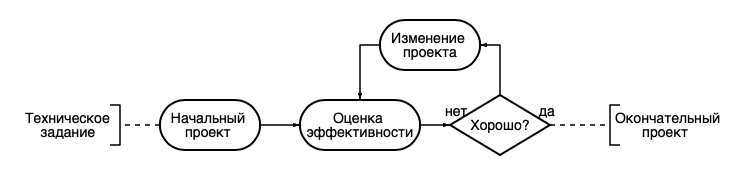
\includegraphics[height =15 cm, keepaspectratio]{images/1_1_1diagram.png}
		\caption{ \textbf{Рис. 2.1.1.} Процесс оптимизации }
	\end{figure}

Алгоритм оптимизации используется для постепенного улучшения проекта до тех пор, пока проект больше не может быть улучшен или пока не будет затрачено запланированное время либо превышена предельно допустимая стоимость. Конструктор несет ответственность за анализ результатов процесса оптимизации, чтобы обеспечить его пригодность для конечного применения. Неправильные спецификации в постановке задачи, плохой начальный проект и неправильно реализованные или неподходящие алгоритмы оптимизации могут привести к неоптимальным или опасным проектам.

Есть несколько преимуществ оптимизации подхода к проектированию. Прежде всего, процесс оптимизации обеспечивает систематическую, логичную процедуру проектирования. При ее правильном соблюдении алгоритмы оптимизации могут уменьшить вероятность ошибки человека при проектировании. Интуиция в инженерном проектировании может ввести в заблуждение; намного лучше оптимизировать данные. Оптимизация может ускорить процесс проектирования, особенно когда процедура может быть написана один раз, а затем повторно применена к другим задачам. Традиционные инженерные методы часто визуализируются и обосновываются людьми в двух или трех измерениях. B то же время современные методы оптимизации могут применяться к задачам с миллионами переменных и ограничений.
   
Есть также проблемы, связанные с использованием оптимизации для проектирования. Мы обычно ограничены в наших вычислительных ресурсах и времени, и поэтому наши алгоритмы должны быть избирательными в том, как они исследуют пространство проектных параметров. По сути, алгоритмы оптимизации ограничены способностью конструктора формулировать задачу. B некоторых случаях алгоритм оптимизации может использовать ошибки моделирования или найти решение, которое не позволяет адекватно решить поставленную задачу. Когда алгоритм приводит к оптимальному проекту, который противоречит интуиции, его может быть трудно интерпретировать. Другое ограничение заключается в том, что многие алгоритмы оптимизации не всегда гарантируют получение оптимальных проектов. 

\section{Математическое определение задачи оптимизации}

Основная задача оптимизации формулируется следующим образом:

\begin{equation}
  \min_{x} \, f(x) 
\end{equation}

\begin{center}
при условии, что $x \in X$
\end{center}

Здесь $x$ — расчетная точка (design point). Расчетная точка мохет быть представлена как вектор значений, соответствующих различным расчетным переменным (design variables). Расчетная точка в $n$-мерном пространстве записывается следующим образом:

\begin{equation}
    [x_1,x_2,...,x_n],
\end{equation}

где $i$-я расчетная переменная обозначена $x_i$. Элементы в этом векторе можно регулировать, чтобы минимизировать целевую функцию $f$. Любое значение $x$ из всех точек в допустимом множестве $F$, которое минимизирует целевую функцию, называется решением или точкой минимума. Конкретное решение записывается как $x^*$. Пример задачи одномерной оптимизации показан на рис. 2.2.1

\begin{figure}[ht]
 \centering
		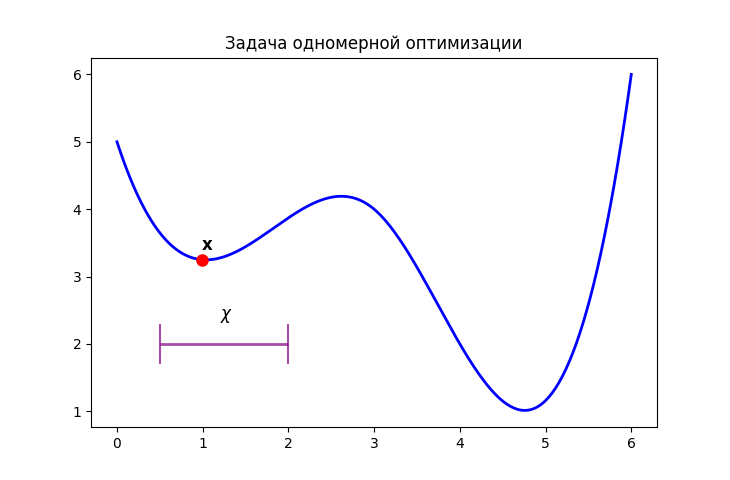
\includegraphics[height =6 cm, keepaspectratio]{images/Figure_1.png}
		\caption{ \textbf{Рис. 2.2.1} Минимум является лучшим вариантом в возможном наборе —
вне допустимой области могут существовать точки с более низкими значениями
}
	\end{figure}

Эта формулировка является общей, т.е. любая задача оптимизации может быть переписана в соответствии с уравнением (2.1.1). B частности, задачу

\begin{equation}
  \min_{x} \, f(x) 
\end{equation}

\begin{center}
при условии, что $x \in X$
\end{center}

можно переформулировать так:

\begin{equation}
  \max_{x} \, -f(x) 
\end{equation}

 \begin{center}
 при условии, что $x \in X$
 \end{center}
 
Задача в новой формулировке имеет тот же самый набор решений. Моделирование инженерных задач в рамках этой математической формулировки может быть сложной задачей. То, как формулируется задача оптимизации, может сделать процесс решения простым или сложным. Следует задаться вопросом какой алгоритм лучше. Если один алгоритм работает лучше, чем другой алгоритм для одного класса задач, то он будет работать хуже для другого класса задач. Чтобы многие алгоритмы оптимизации работали эффективно, в целевой функции должна быть некоторая регулярность, например липшиц-непрерывность или выпуклость. 

\section{Ограничения}

Многие задачи имеют ограничения. Каждое ограничение выделяет множество возможных решений, и в совокупности ограничения определяют допустимое множество  $F$. Допустимые расчетные точки не нарушают никаких ограничений. Например, рассмотрим следующую проблему оптимизации:

\begin{equation}
\min_{x_1, x_2} f(x_1, x_2) 
\end{equation}


 \begin{center}
 при условии, что 
\begin{equation}
  \begin{aligned}
    x_1 &\geq  \\
    x_2 &\geq 0  \\
    x_1 + x_2 &\leq 1
  \end{aligned}
\end{equation}
\end{center}

Допустимое множество изображено на рис. 1.5.1

\begin{figure}[ht]
 \centering
		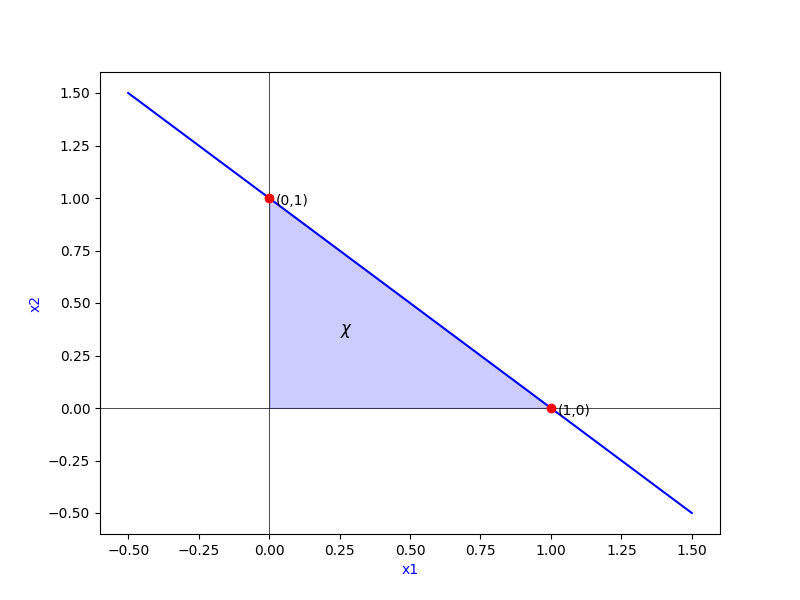
\includegraphics[height =10 cm, keepaspectratio]{images/Figure_2.png}
		\caption{ \textbf{Рис. 2.3.1} Допустимое множество F, заданное неравенствами (2.6) }
	\end{figure}
    
Ограничения обычно записываются с помощью знаков $\leq$, $\geq$ или $=$. Если ограничения включают знаки $<$ или $>$ (т.е. строгие неравенства), то допустимое множество не включает границу ограничений. Потенциальная проблема, которая может возникнуть без учета границы иллюстрируется следующей задачей:


\begin{equation}
  \min_{x} \, x 
\end{equation}

 \begin{center}
 при условии, что $x>1$
 \end{center}

 Допустимое множество показано на рис. 2.3.2. Точка $x = 1$ меньше любого $x$, превышающего единицу, но значение $x = 1$ недопустимо. Можно выбрать любой $x$, произвольно близкий к единице, но превышающей ее, и независимо от того, что выбирать, всегда можно найти бесконечное количество значений, которые расположены еще ближе к единице. Необходимо констатировать, что задача не имеет решения. Чтобы избежать таких проблем, часто лучше включать границу ограничений в допустимое множество.


\begin{figure}[ht]
 \centering
		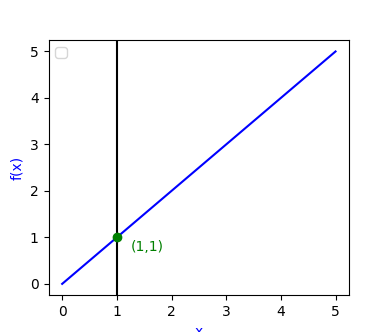
\includegraphics[height =6 cm, keepaspectratio]{images/Figure_3.png}
		\caption{ \textbf{Рис. 2.3.2} Задача (2.7) не имеет решения, поскольку граница ограничения недопустима }
	\end{figure}
    
\section{Критические точки}

На рис. 2.4.1 показана одномерная функция $f(x)$ с несколькими помеченными критическими точками, в которых производная равна нулю и которые представляют интерес при обсуждении задач оптимизации. При минимизации функции $f$ желательно найти точку глобального минимума, т.е. значение $x$, в котором значение $f(x)$ является минимальным. Функция может иметь не более одного глобального минимума, но может иметь несколько точек глобального минимума.

Как правило, трудно доказать, что данная точка-кандидат является точкой глобального минимума. Часто лучшее, что можно сделать, это проверить, соответствует ли она локальному минимуму. Точка $x^*$ является точкой локального минимума, если существует число $\delta > 0$ такое, что $f(x^*) \leq f(x)$ для всех $x$, удовлетворяющих условию $| x - x^*| < \delta$. B многомерном контексте это определение сводится к существованию числа $\delta > 0$ такого, что $f(x^*) \leq f (x)$ для всех $x$, удовлетворяющих условию $||x - x^*|| < \delta$.
На рис. 2.4.1 показаны два типа локальных минимумов: сильный и слабый. Точка сильного локального минимума, которая также называется точкой строгого локального минимума, — это точка, которая однозначно минимизирует $f$ в окрестности. Иначе говоря, точка $x^*$ является точкой строгого локального минимума, если существует число $\delta > 0$ такое, что $f(x^*) < f(x)$ всякий раз, когда $x^* \neq x$ и $||x - x^*|| < \delta$. B многомерном контексте это определение сводится к существованию числа $\delta > 0$ такого, что $f(x^*)< f(x)$всякийраз,когда $x^* \neq x$ и $||x - x^*||< \delta$. Точка слабого локального минимума — это точка локального минимума, которая не является точкой сильного локального минимума.

\begin{figure}[ht]
 \centering
		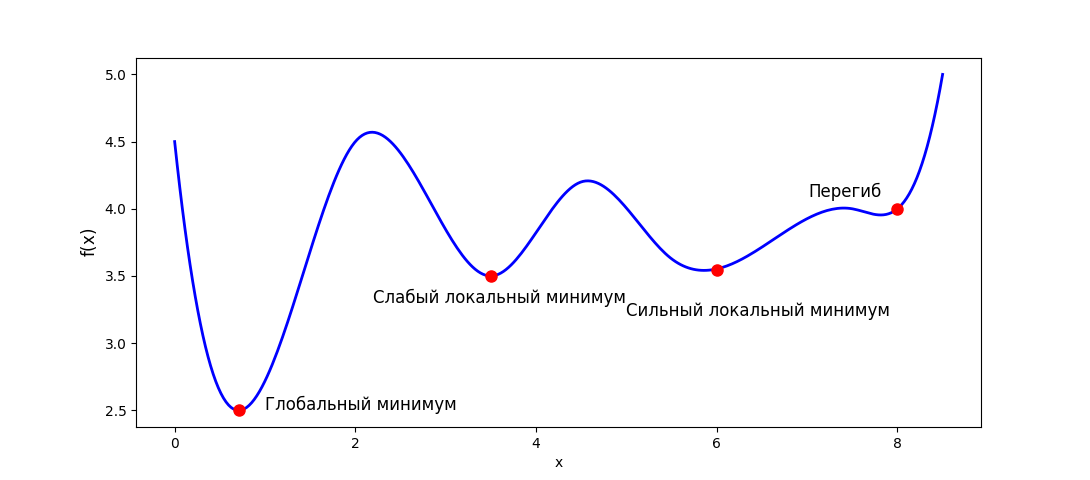
\includegraphics[height =15 cm, keepaspectratio]{images/Figure_4.png}
		\caption{ \textbf{Рис. 2.4.1} Примеры критических точек одномерной функции, представляющих интерес для алгоритмов оптимизации (в которых производная равна нулю)
 }
	\end{figure}
    
Bо всех точках локального и глобального минимума производная непрерывной неограниченной целевой функции равна нулю. Равенство производной нулю — необходимое, но не достаточное условие для локального минимума.
На рис. 2.4.1 показана точка перегиба, где производная равна нулю, но эта точка не является точкой локального минимума функции $f$. Точка перегиба — это место, где меняется знак второй производной функции $f$, что соответствует локальному минимуму или максимуму ее первой производной $f '$. Производная в точке перегиба не обязательно равна нулю.

\printbibliography[title= Список использованных источников]
\end{document}
